\section{Dwi Septiani Tsaniyah{1174003}}

\subsection{Pengertian}
Istilah pada sistem informasi sistem geografis adalah untuk digunakan sebagai pendekatan sebuah sistem yang digunakan dalam sistem informasi geografis , dengan lingkungan yang komponen nya terpisah-pisah,sistem yang digunakan untuk mempermudah pemahaman yang terintegrasi. Pada saat ini teknologi komputer sangat banyak digunakan oleh banyak orang jadi hampir semua sistem informasi nya berdasarkan dengan pada komputer.
Kata informasi berasal dari sebuah pengolahan sejumlah data, di dalam sistem informasi geografis informasi mempunyai volume yang sangat besa. Pada setiap objek geografi memiliki settingan data yang berbeda beda , data tersendiri karena tidak sepenuhnya data yang ada terdapat di dalam peta. Jadi semua data harus diasosiasikan terlebih dahulu untuk menjadi peta yang inteligent, pada data tersebut mampu menampilakn atau memberikan sebuah informasi dengan hanya mengklik mouse pada suatu objek.
Pada istilah geografi ini digunakan karena sistem informasi geografis yang dibangun secara berdasarkan pada geografi. Pada objek ini lebih mengarah pada sfesifikasi lokasi. Objek ini bisa berupa fisik,budaya ataupun ekonomi alamiah. Pada objek ini penampakan nya bisa dilihat didalam sebuah peta yang dimana untuk memberikan sebuah gambaran yang refresentatif dari suatu objek yang sesuai dengan kenyataan di bumi. Pada saat ini teknologi telah membantu proses pemetaan.

\subsection{Sejarah}
Sejarah geografi dimulai sejak manusia mulai berinteraksi dengan lingkunganya, hal ini juga merupakan awal mula dari berkembangnya ilmu pengetahuan tentang geografi.
Pada awal dikenalnya sistem informasi geografis bahwa tidak lepas dari adanya kemajuan didalam bidang teknologi. Pada awal tahun 1960 perkembangan sistem informasi geografis dalam ilmu komputer semakin pesat dan siap dingunakan pada bidang milliter. Pada taun 1700 teknik yang digunakan pada survei modern untuk pemetaan topografis digunakan atau diterapkan , hal ini juga termasuk pada versi awal pemetaan tematis.

\subsection{Koordinat}
Koordinat adalah suatu titik yang didapatkan dari hasil perpotongan dari garis latitude (lintang) dengan garis bujur (longitude) sehingga akan menunjukan lokasi pada suatu daerah. Umumnya koordinat dibedakan menjadi koordinat Geographic dan Universal Transver Mercator (UTM). Pada Koordinat Geogprahic dibedakan menjadi tiga berdasarkan satuannya yaitu :
Koordinat adalah suatu titik yang didapatkan dari hasil pemotongan sebuah garis lintang dengan garis bujur sehingga akan menunjukan sebuah lokasi pada suatu daerah. Pada Bujur/Longitude (X) merupakan garis yang perpindahannya secara vertical dan pada Lintang/Lattitude (Y) merupakan garis yang mempunyai perpindahan secara horizontal, pada (Gambar 1) menjelaskan perpotongan antara garis bujur dan garis lintang akan membentuk suatu titik pertemuan yang biasa disebut dengan titik koordinat.
dibedakan menajadi 3 yaitu : 
\begin{itemize}
	\item Degree, Decimal(DD, DDDD) contoh S 4.56734 E 102.67235
	\item Degree,Minute(DD MM,MMMM) contoh S 4 42,5423’ E 105 34,6445’
	\item Degree, Minute, Second(DD MM SS,SS) contoh : S 4 43’ 45,22 E 103 33’ 33,25
\end{itemize}
\hfill\break
\begin{figure}[H]
	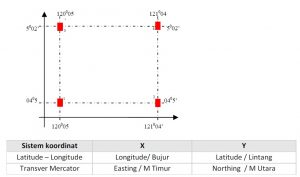
\includegraphics[width=4cm]{figures/1174003/koordinat.jpg}
	\centering
	\caption{Contoh Koordinat}
\end{figure}

\subsection{Data Geospasial}
Geospital data tentang suatu aspek fisik dari sebuah objek yang geografis , misalnya seperti bentuk alam tentu saja sungai,danau,pantai dan bentuk alam lainnya. Secara umun terdapat 2 fitur untuk menampilkan yaitu termasuk ke dalam geografis dan sistem informasi geospasial. Dalam struktur data yang demikian didalam nya ada unsur resolusi sebagai ukuran dari dimensi fitur geografis
Data Geospasial dibagi menjadi 2 yaitu :
\begin{itemize}
	\item Vektor
	Vektor merupakan salah jenis gambar yang dapat dibuat menggunakan aplikasi corel / adobe illustrator / aplikasi vektor lainnya.
	Vektor itu sering digunakan untuk membuat gambar animasi dan vektor juga digunakan oleh goole maps.
	\item Roshen
	Roshen merupakan gambar yang di ambil dari satelit di luar angkasa, gambar ini biasanya bertipe jpg, dan pembaharuan data gambar ini berlangsung lama karena proses nya yang memakan waktu cukup banyak, jenis data ini digunakan oleh google earth.
\end{itemize}
\subsection{Link}
\begin{itemize}
	\item \href{https://youtu.be/CXKVVDaUo30}{Materi GIS}
\end{itemize}
\subsection{Plagiarism}
\begin{figure}[H]
	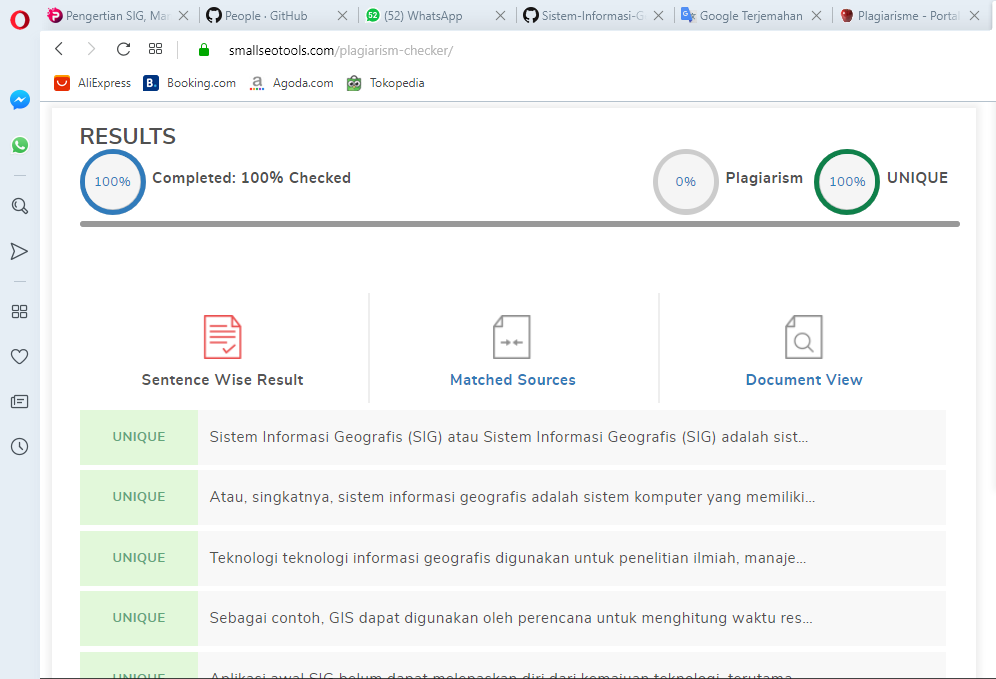
\includegraphics[width=4cm]{figures/1174003/1174003_plagiarisme.png}
	\centering
	\caption{Bukti Tidak Melakukan Plagiat}
\end{figure}